\documentclass[25pt, a1paper, portrait]{tikzposter}
\usepackage[utf8]{inputenc}
 
\title{Atomistic Simulation of Oxygen-Dislocation interaction in Ti alloys.}
\author{Tigany Zarrouk}
\date{\today}
\institute{King's College London}
 
\usepackage{comment}
 
\usetheme{Board}
 
\begin{document}
 
\maketitle
 
\block{~}
{
 Introduction?
}
  
\begin{columns}
    \column{0.4}
    \block{* Main question }{

- How does oxygen play a role in solution hardening in Ti alloys?
- Dislocations are defects that have an atomistic origin. They are line
  defects. 
- How does atomic oxygen interfere with dislocations which in turn changes how
  the plasticity of titanium as a whole?
- Screw dislocations are the most important as they have the least mobility in
  hcp.
}
 
    \column{0.6}
    \block{* Method}{


- Need quantum mechanical method such that we can describe the directionality
  of the bonding sufficiently and obtain accurate forces in the core of the
  dislocation (which determines how the dislocation moves).
- Also this means that the energy orderng of the polymorphs of Ti are
  reproduced. 
- Use TB as quicker than DFT
- Can simulate extended defects due to larger cells, thus mitigating finite
  size effects of simulation due to insufficent relaxation of the dislocation
  core. 
- Built model with optimisation algorithm
\vspace{4cm}}
    \note[
        targetoffsetx=-9cm, 
        targetoffsety=-6.5cm, 
        width=0.5\linewidth
        ]
        {e-mail \texttt{tigany.zarrouk@kcl.ac.uk}}
\end{columns}
 
\begin{columns}
    \column{0.5}
    \block{A figure}
    {
        \begin{tikzfigure}
            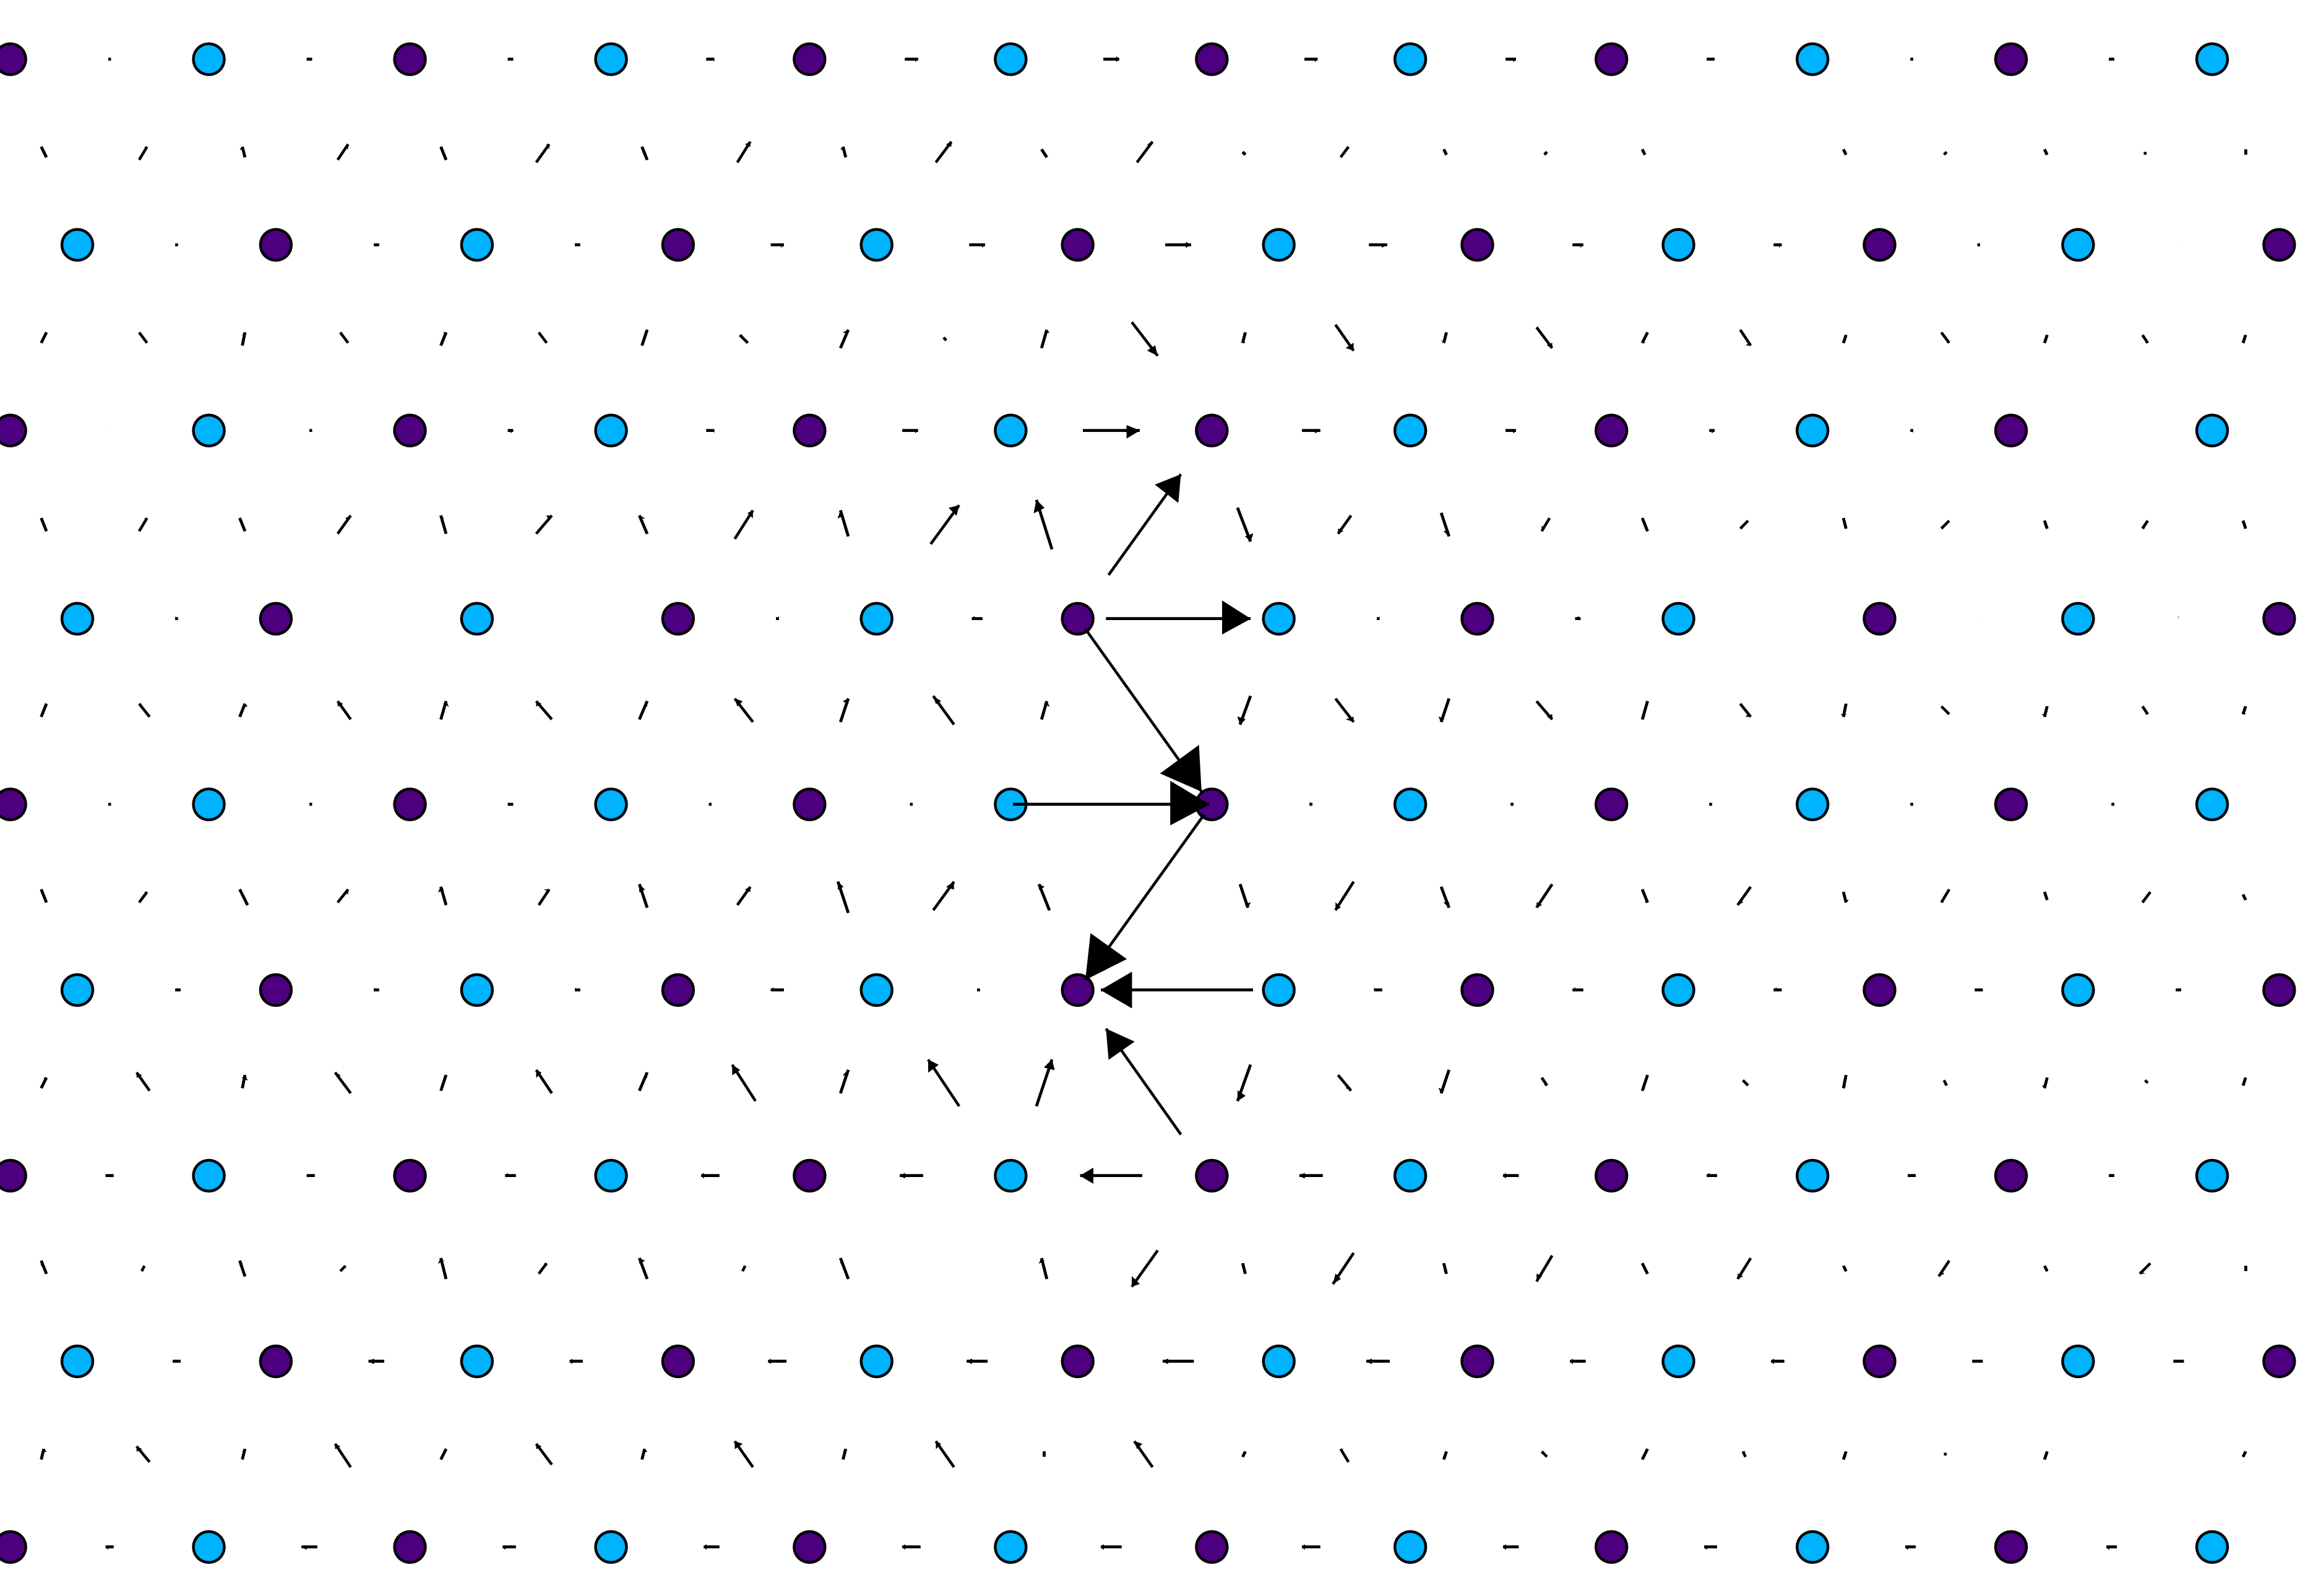
\includegraphics[width=0.4\textwidth]{../Images/zoom_core_look.png}
        \end{tikzfigure}
    }
    \column{0.5}
    \block{Relaxed core of a dislocation in an 'S' quadrupolar
    configuration.}{Relaxed core of this dislocation matches very well with
    literature. ***  See Ghazisaeidi and Trinkle  ***}
\end{columns}


\block{ 
* What are the results
- Want to show how model reproduces core dislocation structure.
- Maybe show how well model fits certain quantities in the fitting? 
- Agrees well with DFT
- Gamma surfaces look reasonable (morphologically speaking: just pretty and
  nothing else really) 
- Going to extend model to add oxygen. 
* What are the implications
}

\end{document}


%%% Local Variables:
%%% mode: plain-tex
%%% TeX-master: t
%%% End:
